\documentclass[tikz]{standalone}
\newcommand*{\AW}[1]{\AA{}\&{}W #1}

\begin{document}
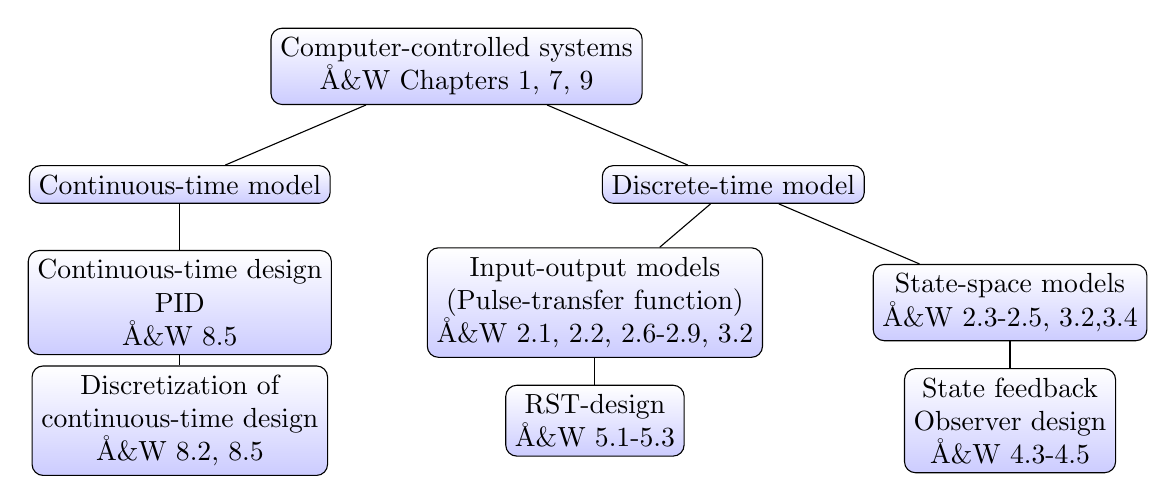
\begin{tikzpicture}[sibling distance=20em,
  every node/.style = {shape=rectangle, rounded corners,
    draw, align=center,
    top color=white, bottom color=blue!20}]]
  \node {Computer-controlled systems\\ \AW{Chapters 1, 7, 9}}
  child { node {Continuous-time model} 
    child { node {Continuous-time design\\PID\\ \AW{8.5} } 
      child { node {Discretization of\\continuous-time design\\ \AW{8.2, 8.5}} 
      } 
    }
  }
  child { node {Discrete-time model}
    child[sibling distance=10em] { node {Input-output models\\(Pulse-transfer function)\\ \AW{2.1, 2.2, 2.6-2.9, 3.2} }
      child { node {RST-design\\ \AW{5.1-5.3} } } }
    child { node {State-space models\\ \AW{2.3-2.5, 3.2,3.4}}
      child { node {State feedback\\Observer design\\ \AW{4.3-4.5} } } 
    }
  };
\end{tikzpicture}
\end{document}
